\section{Specyfikacja wymaganych urządzeń technicznycH}

Aby pełni korzystać z usługi internetu mobilnego oferowanej przez operatora Plus, klient powinien spełnić kilka podstawowych wymagań oraz uwzględnić określone aspekty:

\begin{itemize}
    \item \textbf{Urzadzenie˛ Mobilne}: Klient będzie potrzebował odpowiedniego urządzenia mobilnego, które umożliwi dostęp do internetu mobilnego. Wybór urządzenia może obejmować smartfon, tablet lub modem USB/router mobilny.
    \item \textbf{Karta SIM od Plus}: Karta SIM (Subscriber Identity Module) od operatora Plus jest niezbędna do identyfikacji klienta w sieci oraz umożliwia dostęp do usług operatora. Karta SIM zawiera informacje o numerze telefonu i abonencie, które są niezbędne do zestawienia połączenia z siecią Plus.
    \item \textbf{Oprogramowanie Dostarczone przez Operatora}: W niektórych przypadkach, w zależności od wybranego urządzenia i technologii, operator Plus może dostarczać specjalne oprogramowanie, które ułatwia konfigurację i obsługę usługi internetu mobilnego. To oprogramowanie może być niezbędne do poprawnego działania usługi i powinno być zainstalowane na urządzeniu klienta.
    \item \textbf{Dostęp do Zasięgu Sieci Operatora}: Aby korzystać z usługi internetu mobilnego operatora Plus, klient musi być w zasięgu sieci operatora. Dostępność usługi może być ograniczona w niektórych obszarach, dlatego ważne jest, aby klient sprawdził, czy znajduje się w zasięgu sieci Plus, zanim zdecyduje się na korzystanie z usługi.
    \item \textbf{Wymagania dla Sieci 5G}: W przypadku korzystania z usługi internetu mobilnego w technologii 5G, klient musi spełnić dodatkowe wymagania. Klient będzie potrzebował urządzenia mobilnego lub modemu obsługującego technologię 5G oraz kartę SIM umożliwiającą korzystanie z tej technologii. Warto zauważyć, że technologia 5G oferuje wyższe prędkości i niższe opóźnienia w porównaniu do poprzednich generacji technologii, co sprawia, że jest atrakcyjną opcją dla klientów wymagających szybkiego i niezawodnego dostępu do internetu mobilnego.
\end{itemize}


\begin{figure}[!htb]
    \centering
    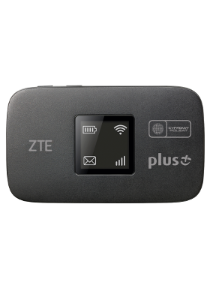
\includegraphics[width=0.2\textwidth]{zte}
    \caption{ZTE MF971R - Router bezprzewodowy z modemem 4G  }
\end{figure}
